\documentclass{ximera}

\newcommand{\RR}{\mathbb R}
\renewcommand{\d}{\,d}
\newcommand{\dd}[2][]{\frac{d #1}{d #2}}
\renewcommand{\l}{\ell}
\newcommand{\ddx}{\frac{d}{dx}}
\newcommand{\dfn}{\textbf}
\newcommand{\eval}[1]{\bigg[ #1 \bigg]}


\outcome{Understand the definiton of a multiple integral.}

\outcome{Use iterated integrals to compute multiple integrals.}

\outcome{Apply Fubini's Theorem.}

\title[Dig-In:]{Integrals with trivial integrands}

\begin{document}
\begin{abstract}
  We study integrals over general regions with and integrand equaling one.
\end{abstract}
\maketitle


Now we will integrate over regions that are more complex than
rectangles and boxes. In particular we will find areas of regions
bounded by curves in $\R^2$, and volumes of regions bounded by
surfaces in $\R^3$.

\section{Double integrals and area}

We start with Fubini's Theorem. While we will state it generally, in
this section the integrand, $F$, will always be $1$.

\begin{theorem}[Fubini's Theorem]\index{Fubini's Theorem}
  Let $R$ be a closed, bounded region in the $(x,y)$-plane and let
  $F(x,y)$ be a continuous function on $R$.
  \begin{itemize}
  \item If
    \[
    R=\{(x,y):\text{$a\leq x\leq b$ and $g_1(x)\leq y\leq g_2(x)$}\}
    \]
    where $g_1$ and $g_2$ are continuous functions on $[a,b]$, then
    \[
    \iint_R F(x,y) \d A = \int_a^b\int_{g_1(x)}^{g_2(x)} F(x,y)\d y\d x.
    \]
  \item If
    \[
    R=\{(x,y):\text{$c\leq y\leq d$ and $g_1(y)\leq x\leq g_2(y)$}\}
    \]
    where $g_1$ and $g_2$ are continuous functions on $[c,d]$, then
    \[
    \iint_R F(x,y)\d A = \int_c^d\int_{g_1(y)}^{g_2(y)} F(x,y)\d x\d y.
    \]
\end{itemize}
\end{theorem}

When the integrand of a double integral is $1$, like this
\[
\iint_R\d A
\]
this integral computes the \textbf{area} of the region. This is
because you are finding the ``signed volume'' between the curve and
the plane $z=1$. In our first example, we will use this ``hammer to
swat a fly,'' meaning, we are essentially using a much more difficult
method than necessary! We apologize in advance, and include the
example because it is illustrative of the method of using double
integrals to compute areas.

\begin{example}
  Set-up and evaluate a double integral that will compute the area of
  the region below:
  \begin{image}
    \begin{tikzpicture}
      \begin{axis}[
          tick label style={font=\scriptsize},
          axis y line=middle,axis x line=middle,
          axis on top,name=myplot,
	  xtick={1,2,3},
	  ytick={1,2,3},
	  ymin=-.5,ymax=2.5,%
	  xmin=-.5,xmax=3.5,
          rounded corners=.5pt
        ]
        \draw [ultra thick,penColor] (axis cs:1,1) -- (axis cs: 3,1)-- (axis cs: 1,2)  -- cycle;
        
        \draw (axis cs: 1.5,1.3) node {$R$};
      \end{axis}
      
      \node [right] at (myplot.right of origin) {\scriptsize $x$};
      \node [above] at (myplot.above origin) {\scriptsize $y$};
    \end{tikzpicture}
  \end{image}
  \begin{explanation}
    Our region above can be defined by:
    \[
    R=\{(x,y):\text{$1\leq x\leq 3$ and $1\leq y\leq -x/2+5/2$}\}
    \]
    The area of this region is given by, write with me, 
    \begin{align*}
      \int_{\answer[given]{1}}^{\answer[given]{3}}\int_{\answer[given]{1}}^{\answer[given]{-x/2+5/2}}\d y \d x &= \int_{\answer[given]{1}}^{\answer[given]{3}} \eval{\answer[given]{y}}_{\answer[given]{1}}^{\answer[given]{-x/2+5/2}} \d x\\
      &=  \int_{\answer[given]{1}}^{\answer[given]{3}} \left(\answer[given]{-x/2+3/2}\right) \d x\\
      &=  \eval{\answer[given]{-x^2/4+3x/2}}_{\answer[given]{1}}^{\answer[given]{3}}\\
      &= \answer[given]{1}. 
    \end{align*}
  \end{explanation}
\end{example}

\begin{question}
  In the previous example, we integrated with respect to $y$
  first. Set-up an integral that computes the area of $R$ that
  integrates with respect to $x$ first.
  \begin{prompt}
    Start by finding overall bounds for our variables. In this case:
    \begin{align*}
      1\le &x \le 3\\
      1\le &y \le -x/2 + 5/2 \le \answer{2}
    \end{align*}
    Now, write $x$ in terms of $y$. Write with me:
    \begin{align*}
      \answer{-3/2}\le &y -5/2 \le -x/2  \le \answer{-1/2}\\
      \answer{1/2}\le &x/2 \le 5/2-y  \le \answer{3/2}\\
      1\le & x\le \answer{5-2y}  \le 3
    \end{align*}
    We may now write our desired integral:
    \[
    \iint_R \d A = \int_{\answer{1}}^{\answer{2}}\int_{\answer{1}}^{\answer{5-2y}} \d x \d y
    \]
  \end{prompt}
\end{question}

In our example above, we used an integral to find the area of a
triangle. Whenever you learn a new technique, you should always ``try
it out'' on a computation where you know the answer through a
different method. With our next two examples, we'll work with regions
where calculus really helps out.

\begin{example}
  Set-up and evaluate a double integral that will compute the area of
  the region below:
  \begin{image}
    \begin{tikzpicture}
      \begin{axis}[
          tick label style={font=\scriptsize},axis y line=middle,axis x line=middle,name=myplot,axis on top,%
	  xtick={2,4,...,12},
	  ytick={-2,-4,-6,6,4,2},
	  ymin=-6.9,ymax=6.9,%
	  xmin=-.5,xmax=12.9%
        ]
        \draw (axis cs: 6,2) node {$R$}
	(axis cs: 4,4.5) node [rotate=23] {\scriptsize $x=y^2/3$};
        
        \addplot [penColor,ultra thick, smooth,domain=-6:6,samples=20] ({x^2/3},{x}) -- cycle;
      \end{axis}
      \node [right] at (myplot.right of origin) {\scriptsize $x$};
      \node [above] at (myplot.above origin) {\scriptsize $y$};
    \end{tikzpicture}
  \end{image}
  \begin{explanation}
    Our region above can be defined by:
    \[
    R=\{(x,y):\text{$-6\leq y\leq 6$ and $y^2/3\leq x\leq 12$}\}
    \]
    The area of this region is given by, write with me, 
    \begin{align*}
      \int_{\answer[given]{-6}}^{\answer[given]{6}}\int_{\answer[given]{y^2/3}}^{\answer[given]{12}}\d x \d y &= \int_{\answer[given]{-6}}^{\answer[given]{6}} \eval{\answer[given]{x}}_{\answer[given]{y^2/3}}^{\answer[given]{12}} \d y\\
      &=  \int_{\answer[given]{-6}}^{\answer[given]{6}} \left(\answer[given]{12-y^2/3}\right) \d y\\
      &=  \eval{\answer[given]{12y-y^3/9}}_{\answer[given]{-6}}^{\answer[given]{6}}\\
      &= \answer[given]{96}. 
    \end{align*}
  \end{explanation}
\end{example}

\begin{question}
  In the previous example, we integrated with respect to $x$
  first. Set-up an integral that computes the area of $R$ that
  integrates with respect to $y$ first.
  \begin{prompt}
    Start by finding overall bounds for our variables. In this case:
    \begin{align*}
      \answer{0}\le y^2/3\le &x \le 12\\
      -6\le &y \le 6
    \end{align*}
    Now, write $y$ in terms of $x$. Write with me:
    \begin{align*}
      \answer{0}\le &y^2 \le 3x \le \answer{36}\\
      \answer{-6}\le -\sqrt{3x}\le &y \le \sqrt{3x} \le \answer{6}\\
      1\le & x\le \answer{5-2y}  \le 3
    \end{align*}
    We may now write our desired integral:
    \[
    \iint_R \d A = \int_{\answer{0}}^{\answer{12}}\int_{\answer{-\sqrt{3x}}}^{\answer{\sqrt{3x}}} \d y \d x
    \]
  \end{prompt}
\end{question}

And now for one more example of using a double integral to compute the
area of a region.

\begin{example}
  Set-up and evaluate a double integral that will compute the area of
  the region below:
  \begin{image}
    \begin{tikzpicture}
      \begin{axis}[
          tick label style={font=\scriptsize},axis y line=middle,axis x line=middle,name=myplot,axis on top,%
	  ymin=-.5,ymax=1.1,%
	  xmin=-.5,xmax=1.1%
        ]
        \draw (axis cs: .5,.4) node {$R$}
	(axis cs: .5,.8) node [rotate=26] {\scriptsize $y=\sqrt{x}$}
	(axis cs: .75,.16) node [rotate=29] {\scriptsize $y=x^4$};
        
        \addplot [penColor,ultra thick, smooth,domain=0:1.05,samples=20] ({x},{x^4});
        \addplot [penColor,ultra thick, smooth,domain=0:1.05,samples=20] ({x^2},{x});
      \end{axis}
      
      \node [right] at (myplot.right of origin) {\scriptsize $x$};
      \node [above] at (myplot.above origin) {\scriptsize $y$};
    \end{tikzpicture}
  \end{image}
  \begin{explanation}
    Our region above can be defined by:
    \[
    R=\{(x,y):\text{$0\leq x\leq 1$ and $x^4\leq y\leq \sqrt{x}$}\}
    \]
    The area of this region is given by, write with me, 
    \begin{align*}
      \int_{\answer[given]{0}}^{\answer[given]{1}}\int_{\answer[given]{x^4}}^{\answer[given]{\sqrt{x}}}\d y \d x &= \int_{\answer[given]{0}}^{\answer[given]{1}} \eval{\answer[given]{y}}_{\answer[given]{x^4}}^{\answer[given]{\sqrt{x}}} \d x\\
      &=  \int_{\answer[given]{0}}^{\answer[given]{1}} \left(\answer[given]{\sqrt{x}-x^4}\right) \d x\\
      &=  \eval{\answer[given]{2x^{3/2}/3 - x^5/5}}_{\answer[given]{0}}^{\answer[given]{1}}\\
      &= \answer[given]{7/15}. 
    \end{align*}
  \end{explanation}
\end{example}

\begin{question}
  In the previous example, we integrated with respect to $y$
  first. Set-up an integral that computes the area of $R$ that
  integrates with respect to $x$ first.
  \begin{prompt}
    Start by finding overall bounds for our variables. In this case:
    \begin{align*}
      0\le &x \le 1\\
      \answer{0}\le x^4\le &y \le \sqrt{x}\le \answer{1}
    \end{align*}
    Now, write $x$ in terms of $y$. Since $y$ is bounded by $x$ on
    both sides, we'll do this in two steps. Write with me:
    \begin{align*}
      \answer{0}\le &x^4\le y\\
      0 \le &x \le \answer{y^{1/4}}
    \end{align*}
    and
    \begin{align*}
      y\le &\sqrt{x}\le \answer{1}\\
      \answer{y^2} \le &x \le 1
    \end{align*}
    We may now write our desired integral:
    \[
    \iint_R \d A = \int_{\answer{0}}^{\answer{1}}\int_{\answer{y^2}}^{\answer{y^{1/4}}} \d x \d y
    \]
  \end{prompt}
\end{question}


\section{Triple integrals and volume}

We start by again(!) introducing another version of Fubini's Theorem.

\begin{theorem}[Fubini]\index{Fubini's Theorem}
  Let $R$ be a closed, bounded region in $\R^3$ and let $F(x,y,z)$ be
  a continuous function on $R$. If
    \begin{align*}
      R=\{(x,y,z):&\text{$a\leq x\leq b$, $g_1(x)\leq y\leq g_2(x)$,}\\
        &\text{and $H_1(x,y) \leq z \leq H_2(x,y)$}\}
    \end{align*}
    where $g_1$ and $g_2$ are continuous functions on $[a,b]$, and $H_1$ and $H_2$ are continuous on the region
    \[
    S =\{(x,y):\text{$a\leq x\leq b$ and $g_1(x)\leq y\leq g_2(x)$}\}
    \]
    then
    \[
    \iiint_R F(x,y,z) \d V = \int_a^b\int_{g_1(x)}^{g_2(x)}\int_{H_1(x,y)}^{H_2(x,y)} F(x,y,z)\d z\d y\d x.
    \]
    There are \textit{six} reorderings total with three variables. We will spare
    the young mathematician the details, and trust that you will sort
    it out.
\end{theorem}

Now with Fubini's help, we will use triple integrals to compute
volumes.

\begin{example}
  Set-up and evaluate a double integral that will compute the volume of
  the region bounded by:
  \begin{itemize}
  \item The plane $x=0$.
  \item The plane $y=0$.
  \item The plane $z=0$.
  \item The plane $3x + 4y + 6z = 12$.
  \end{itemize}
  \begin{explanation}
    Our region above produces a
    \textit{tetrahedron}\index{tetrahedron}, a triangular-based
    pyramid. It intersects the $x$-axis at $(4,0,0)$, the $y$-axis at
    $(0,3,0)$, and the $z$-axis at $(0,0,2)$.  The region can be
    defined by:
    \begin{align*}
      R=\Big\{(x,y,z):&0\leq x\leq 4, \\
      &0\leq y\leq -3x/4+3, \\
      &0\leq z \leq \frac{12-3x-4y}{6}\Big\}
    \end{align*}
    The volume of this region is given by, write with me, 
    \[
    \int_{\answer[given]{0}}^{\answer[given]{4}} \int_{\answer[given]{0}}^{\answer[given]{-3x/4+3}} \int_{\answer[given]{0}}^{\answer[given]{\frac{12-3x-4y}{6}}}\d z \d y\d x 
    \]
    \begin{align*}
      &=\int_{\answer[given]{0}}^{\answer[given]{4}} \int_{\answer[given]{0}}^{\answer[given]{-3x/4+3}} \answer[given]{\frac{12-3x-4y}{6}} \d y \d x\\
      &= \int_{\answer[given]{0}}^{\answer[given]{4}}  \eval{\answer[given]{2y-\frac{xy}{2}-\frac{y^2}{3}}}_{\answer[given]{0}}^{\answer[given]{-3x/4+3}} \d x\\
      &= \int_{\answer[given]{0}}^{\answer[given]{4}}  \left(\answer[given]{\frac{3x^2}{16} -\frac{3x}{2}+3}\right) \d x\\
      &= \eval{\answer[given]{x^3/16-3x^2/4+3x}}_{\answer[given]{0}}^{\answer[given]{4}} \d x\\
      &=\answer[given]{4}.
    \end{align*}    
  \end{explanation}
\end{example}

\begin{question}
  In the previous example, we integrated with respect to $z$, then
  $y$, then $x$. Set-up an integral that computes the volume of $R$
  that integrates with respect to $x$, then $z$, then $y$.
  \begin{prompt}
    %% BABBAD -- double check this is the problem you want to do.
    %% 
    %% Start by finding overall bounds for our variables. In this case:
    %% \begin{align*}
    %%   0\le &x \le 4\\
    %%   0\le &y \le -3x/4+3 \le \answer{3}\\
    %%   0\le &z \le \frac{12-3x-4y}{6}\le \answer{2}
    %% \end{align*}
    %% Now, write $z$ in terms of $y$. Write with me:
    %% \begin{align*}
    %%   \answer{0}\le &x^4\le y\\
    %%   0 \le &x \le \answer{y^{1/4}}
    %% \end{align*}
    %% and
    %% \begin{align*}
    %%   y\le &\sqrt{x}\le \answer{1}\\
    %%   \answer{y^2} \le &x \le 1
    %% \end{align*}
    %% We may now write our desired integral:
    
    \[
    \iiint_R \d V = \int_{\answer{0}}^{\answer{3}}\int_{\answer{0}}^{\answer{-2y/3+2}} \int_{\answer{0}}^{\answer{\frac{12-4y-6z}{3}}} \d x \d z \d y
    \]
  \end{prompt}
\end{question}


\begin{example}
  Set-up a double integral that will compute the volume of the region
  bounded by the cone below:
  \begin{image}
    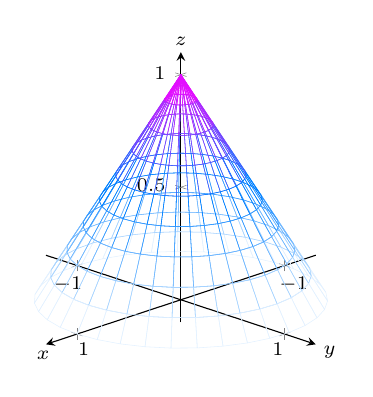
\begin{tikzpicture}
      \begin{axis}%
        [
          tick label style={font=\scriptsize},%axis on top,
	  axis lines=center,
	  view={135}{25},
	  name=myplot,
	  %% xtick=\empty,
	  %% ytick=\empty,
	  %% ztick=\empty,
	  %% extra x ticks={1},
	  %% extra x tick labels={$a$},
	  %% extra y ticks={1},
	  %% extra y tick labels={$a$},
	  %% extra z ticks={1},
	  %% extra z tick labels={$h$},
	  ymin=-1.3,ymax=1.3,
	  xmin=-1.3,xmax=1.3,
	  zmin=-.1, zmax=1.1,
	  every axis x label/.style={at={(axis cs:\pgfkeysvalueof{/pgfplots/xmax},0,0)},xshift=-1pt,yshift=-4pt},
	  xlabel={\scriptsize $x$},
	  every axis y label/.style={at={(axis cs:0,\pgfkeysvalueof{/pgfplots/ymax},0)},xshift=5pt,yshift=-3pt},
	  ylabel={\scriptsize $y$},
	  every axis z label/.style={at={(axis cs:0,0,\pgfkeysvalueof{/pgfplots/zmax})},xshift=0pt,yshift=4pt},
	  zlabel={\scriptsize $z$},colormap/cool
	]
        
        \addplot3[domain=0:1,,y domain=0:360,mesh,samples=10,samples y=36,very thin,z buffer=sort] ({x*cos(y)}, {x*sin(y)},{1-x});
      \end{axis}
    \end{tikzpicture}
  \end{image}
  \begin{explanation}
    First note that 
    \begin{align*}
      R=\{(x,y,z):&\text{$-1\leq x\leq 1$, $-\sqrt{1-x^2}\leq y\leq \sqrt{1-x^2}$}, \\
        &\text{and $0\leq z \leq 1-\sqrt{x^2+y^2}$}\}
    \end{align*}
    Hence, the volume of this region is given by
    \[
    \int_{\answer[given]{-1}}^{\answer[given]{1}}
    \int_{\answer[given]{-\sqrt{1-x^2}}}^{\answer[given]{\sqrt{1-x^2}}}
    \int_{\answer[given]{0}}^{\answer[given]{1-\sqrt{x^2+y^2}}}\d z \d y\d x.
    \]
    \end{explanation}
\end{example}

\begin{question}
  In the previous example, we integrated with respect to $z$, then
  $y$, then $x$. Set-up an integral that computes the volume of $R$
  that integrates with respect to $x$, then $y$, then $z$.
  \begin{prompt}
    \[
    \iiint_R \d V =
    \int_{\answer{0}}^{\answer{1}}
    \int_{\answer{-1+z}}^{\answer{1-z}}
    \int_{\answer{-\sqrt{(1-z)^2-y^2}}}^{\answer{\sqrt{(1-z)^2-y^2}}}
    \d x \d y \d z
    \]
  \end{prompt}
\end{question}

\section{When the integrand isn't one}

What if the integrand isn't $1$? Computationally, you just do what you
did before, but you have an additional antiderivative to
compute. Conceptually, much more can be happening. We'll see this soon.

\end{document}
